\documentclass[11pt]{article}
\usepackage[margin=1in]{geometry}
\usepackage{booktabs}
\usepackage{amsmath,amssymb}
\usepackage{microtype}
\usepackage{graphicx}
\usepackage{float}
\usepackage[hidelinks]{hyperref}
\usepackage{enumitem}
\setlist{itemsep=2pt,topsep=3pt}
\newcommand{\code}[1]{\texttt{#1}}

\title{The Curated Database:\\ from the v2 Function-Keyed Store to the v3 True-Friend Store}
\author{local\_mixing project note}
\date{September 28 -- October 2, 2026}

\begin{document}
\maketitle

\noindent\emph{Summary of the curated-DB redesign: old vs.\ new structure and
operation, the definitional variants, the experimental record, and the
rationale for continuing with modes (c) and (b$'$). Companion artifacts:
\code{CURATED\_DB\_FINDINGS.md} (pre-redesign diagnosis),
\code{runs/ncdb\_ab\_20261001/RESULTS.md} (experiment tables),
\code{runs/ncdb\_random\_20261001/RESULTS.md} (ablation runs).}

\section{Setting}

Stage~3 (\code{db\_mixing}) replaces sampled windows of the circuit with
equivalent spellings drawn from two frozen stores: the \textbf{regular} store
(\code{frozen\_m1\_m11}, the complete g57 replacement corpus through 11
gates, function-keyed) and the \textbf{curated} store, whose job is to offer
\emph{meaningfully different} alternatives for a window---above all,
equal-length re-spellings, the staple of in-place mixing. The redesign
concerns only the curated store; the regular store and the move loop are
unchanged.

\section{The old store (v2, function-keyed)}

\paragraph{Construction} (\code{build\_curated\_full from-frozen-identities-v2}):
\begin{enumerate}[nosep]
\item For every multi-member class of the regular store (9.68M classes:
functions with $\ge 2$ stored spellings $a,b$ of $\le 11$ gates), form the
pair identity $a\cdot\mathrm{rev}(b)$; canonicalize; cancel adjacent
duplicates.
\item Deduplicate identities by dihedral orbit: 20.0M words $\to$ 7.47M
orbits.
\item For each orbit word of length $n$: enumerate every direction $\times$
rotation $\times$ split. Each split $P\,|\,S$ emits \emph{both} $P$ and
$\mathrm{rev}(S)$ under the \emph{function key of the prefix}
(canonical-polynomial hash), rewired into the prefix's canonical wire frame
and gate-canonicalized.
\item Keep one lexicographic representative per (identity, key, gate
count)---the ``sibling collapse''---then byte-exact global dedup.
\end{enumerate}

\paragraph{Shape.} 15.55M keys / 276M candidates. Structural facts
established during the diagnosis: every pair identity simplifies to $\le 12$
gates (multi-member classes concentrate at $\le 6$-gate members; longer
pairings cancel), hence candidates cap at 11 gates; \textbf{keys exist only
for functions of minimal length $\le 6$}; long candidates pile up under
near-trivial keys (the single-gate key held 7.7M spellings, 245\,MB; the
identity-function key 2.6M).

\paragraph{Operation.} The curated-exhaust cascade probes the curated store
first, at every window length, by the window's \emph{function} key (forward
direction); any stored spelling of that function is a candidate; the regular
store is consulted only on a complete curated miss.

\paragraph{Why it failed.}
\begin{itemize}
\item[F1.] \textbf{The sibling collapse was wrong at the midpoint}: there
$P$ and $\mathrm{rev}(S)$ are the two genuinely different halves ($a$ and
$b$), and one was dropped. 48\% of keys held a \emph{single} candidate---
usually the window itself---although a different same-length spelling
provably existed for 95\% of them.
\item[F2.] \textbf{No difference guarantee}: pools mixed rotation debris,
commuting re-spellings, and the window itself; once the canonical-order
identity guard landed, 43\% of moves were re-spelling rejections.
\item[F3.] \textbf{Catastrophic lookup cost}: mean candidates per splice
choice 327k--660k; throughput fell from ${\sim}100$k moves/min to
${\sim}100$k moves per 30--60\,min.
\item[F4.] \textbf{No provenance} for why a candidate suited a window.
\end{itemize}

\section{The new notion: true friends}

With involutive gates, $C^{*}=C^{-1}=\mathrm{rev}(C)$.

\paragraph{Strict definition.} $D$ is a \emph{true friend} of $C$
(spellings of one function $f$, $\delta=\mathrm{minlen}(f)$) when the closed
loop $C\cdot D^{*}$ is \emph{locally minimal except for a sanctioned chord}
between its junctions $\mathrm{ID}$ and $P_f$: for every pair of
prefix-permutations $u,v$ on the loop, the true Cayley distance equals the
arithmetic minimum over the four sanctioned routes (two arcs along the loop;
two routes through a $\delta$-gate geodesic chord). The per-circuit half of
this---every window of $C$ sits exactly on its sanctioned routes---is
\textbf{chord-tightness}; for a geodesic spelling it reduces to classical
local geodesicity, and for a non-minimal spelling it allows exactly the slack
the chord explains. By construction: the two prefix paths never re-meet away
from the junctions, so self-pairs and all commuting reorders are excluded
(F2 dies definitionally); the identity-function key cannot exist; provenance
is the definition itself (F4).

\paragraph{Relativized routes.} When the \emph{key} circuit is not required
to be tight (below), junction routes are priced with proven distances of its
actual prefixes rather than raw gate counts---the original ``shortest path
through $\mathrm{ID}$ or $P_C$'' phrasing; on tight circuits this coincides
with the arithmetic form.

\paragraph{Leeway.} A graded relaxation lets a check miss its sanctioned
minimum by at most $t$ gates, with $t=2$ for pair total length $\ge 9$,
$t=1$ for $7$--$8$, else $0$.

\paragraph{The oracle.} Distances are decided by a layered oracle:
exhaustive exact tables for $\mathrm{minlen}\le 3$ (all 1/2/3-gate words up
to relabelling---$1+31+1{,}639$ functions, cross-validated against the pool
census) plus regular-store members as shortcut witnesses. Checks with
threshold $\le 4$ are exact; above that, a pass means \emph{no shortcut
witnessed}---the same evidence the replacement-db adversary holds. The
layering was forced by a discovery: the regular store is a replacement
table, \emph{not} a minimality oracle (the single-gate function's class
stores only 5- and 6-gate re-spellings).

\section{The new store (v3 ``ncdb'', circuit-keyed)}

\paragraph{Pools.} The v2 enumeration re-ran \emph{without} the sibling
collapse: same 7.47M identities, all exact-distinct arcs kept---779.2M
candidates over the same 15.55M function keys, \textbf{zero
single-candidate pools} (F1 fixed at the source).

\paragraph{Pairs.} One pass over the pools (reservoir $\le 48$ members per
pool $\times$ length, $\le 2{,}500$ pairs per pool; pools $\le 64$
members---96\% of keys---are exhaustive) evaluates each sampled pair under
the layered oracle and emits every qualifying \emph{ordered} pair
$(C\to D)$ into per-mode stores:

\begin{center}
\begin{tabular}{llllrr}
\toprule
mode & key $C$ & friend $D$ & cross & keys & pairs\\
\midrule
a  & tight & tight & exact & 0.44M & 0.83M\\
\textbf{c} & \textbf{unconstrained} & \textbf{tight} & \textbf{exact} & \textbf{1.96M} & \textbf{3.30M}\\
v2 & unconstrained & slack $\le t$, small exact & exact & 2.54M & 5.12M\\
c1 & unconstrained & as b$'$, leeway $\le 1$ & $\le 1$ & 4.33M & 9.42M\\
v1 & unconstrained & tight & $\le t$ & 12.05M & 28.0M\\
\textbf{b$'$} & \textbf{unconstrained} & \textbf{slack $\le t$, win.\ $\le4$ exact} & \textbf{$\le t$} & \textbf{16.87M} & \textbf{63.1M}\\
b  & unconstrained & slack $\le t$ & $\le t$ & 18.73M & 194.2M\\
\bottomrule
\end{tabular}
\end{center}

\noindent Containments: a $\subseteq$ c $\subseteq$ \{v1, v2, c1\}
$\subseteq$ b$'$ $\subseteq$ b. The \emph{unconstrained key} is the
deliberate asymmetry: a junky window should be replaceable by a certified
friend; the relation is therefore directed, and splices drift toward tight
material.

\paragraph{Records and keys.} A record is
$\mathrm{xxh3}_{128}(\text{canonical circuit blob of } C)\,\|\,\text{blob of
} D$: the key is the \emph{circuit}, not the function---different spellings
of one function are different keys, each owning only its certified friends,
stored in the same canonical wire frame the function key would induce (the
decode path is unchanged). Stores are direction-complete, with no
min-direction fold. Friend lists are small by construction: (c) median 1
friend/key (mean 1.68), (b$'$) median 2 (mean 3.74).

\paragraph{Runtime.} \code{FROZEN\_CURATED\_KEY=circuit} switches the
curated stage (and the leakage-repair QC path) to the circuit key, computed
byte-identically to the builder, with a round-trip-verified g57 encoder so
non-g57 windows fail closed to a miss. Decode, selection, guards and splice
are untouched; misses are the common case and cost a Bloom probe
(${\sim}0.39\%$ FP).

\section{The experimental record}

\begin{itemize}
\item \textbf{Probe.} Pool material is ${\sim}85\%$ tight at the
short/geodesic end but $2.5$--$3.5\%$ at 7 gates and ${\sim}0\%$ at 9--11
gates---most of the 779M-candidate mass is dead weight under any mode.
Among tight pairs, strict passes are rare over hard functions
(${\sim}0.8\%$ at $(6,6)$, $\delta=6$) and plentiful over easy ones
(${\sim}80\%$ at $(5,5)$, $\delta\le 2$). The b-vs-b$'$ gap at $\ge 6$-gate
friends is almost entirely friends carrying compressible $\le 4$-gate
windows---the hazard the b$'$ floor removes.
\item \textbf{Full-profile A/B} (mini-sandwich TDP, 3.65M moves, same
seed/binary): both arms finished in \textbf{27 min} (v2-store runs needed
$>1$ day per 1M moves). Mean candidates per choice 1.5--2.2 (vs 327k);
identity-skips at matched 700k moves 232k/224k vs 311k (old baseline) and
593k (old fixed); curated splices are two-thirds \emph{equal-length}
(22k $4{\leftrightarrow}4$ + 27k $5{\leftrightarrow}5$ for (c); 163k
$5{\leftrightarrow}5$ for (b$'$))---the move class v2 could not honestly
serve.
\item \textbf{Ridge vs the old store} (stage-2 rows vs 1M-move states,
identical grids): old 0.3409; (c) 0.3267/0.3334 (two seeds); (b$'$)
0.3348/0.3318.
\begin{figure}[H]
\centering
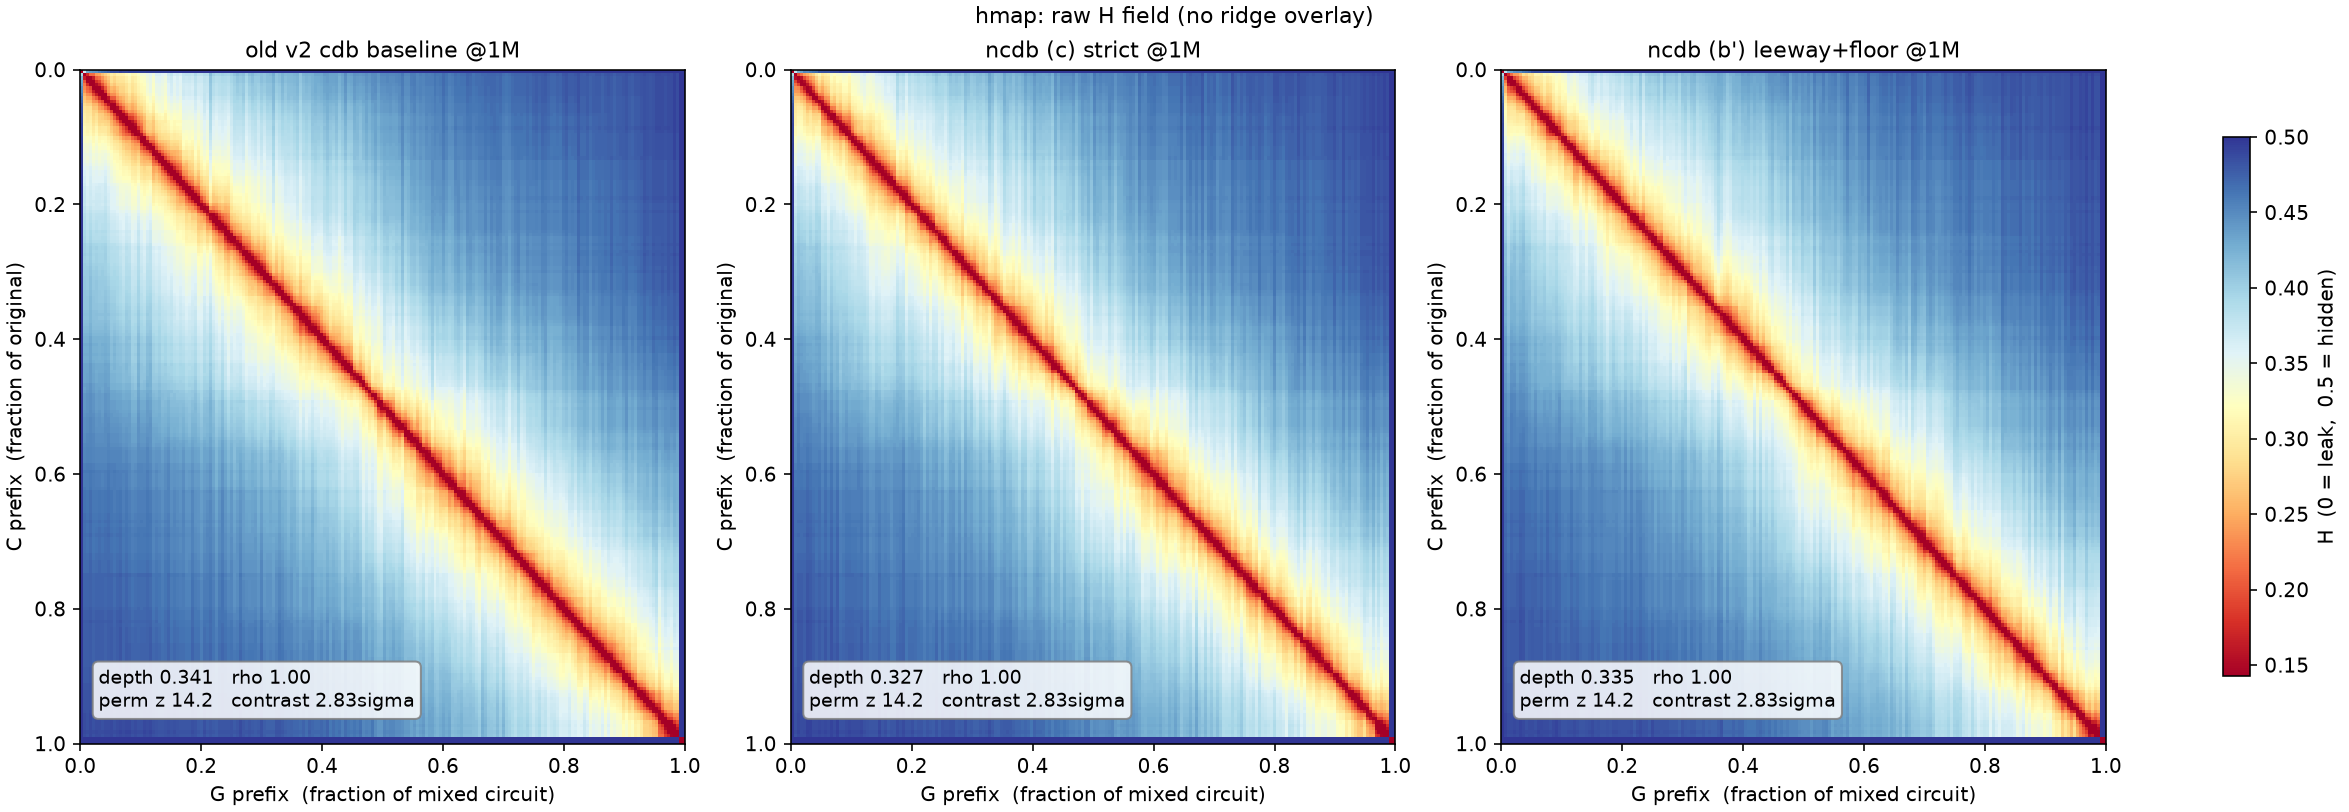
\includegraphics[width=\linewidth]{figures/mv1M_plates.png}
\caption{Three-way 1M-move heatmap plates on identical grids: the old v2
store vs.\ ncdb (c) and (b$'$).}
\end{figure}
\item \textbf{Seed-replicated matrix} (5 stores $\times$ 2 seeds, 1M):
within-store seed spread 0.003--0.007 equals every between-store gap---no
ncdb variant separates from any other; the robust fact is 10/10 ncdb runs
below the old store.
\begin{figure}[H]
\centering
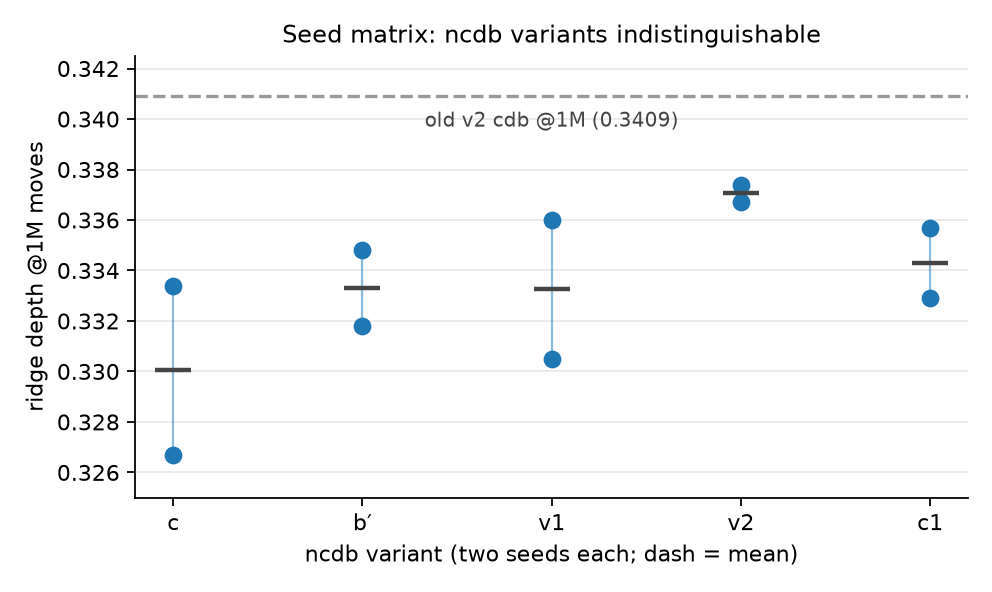
\includegraphics[width=0.82\linewidth]{figures/matrix_dots.png}
\caption{Seed-replicated 1M matrix: each variant's two seeds (dash = mean)
against the old store's depth. Within-store spread equals between-store
gaps.}
\end{figure}
\item \textbf{Expansion-factor sweep} (profile $3,5,5,F,F$ on (c)):
monotone and strong---$F=1.5/2.5/3/5 \to$ depth
$0.3243/0.2997/0.2964/0.2814$, DB-splices $12.2/24.6/29.5/40.5\%$ of moves
($6$--$14\times$ seed noise); re-confirms ``$r$ is the master knob''.
\begin{figure}[H]
\centering
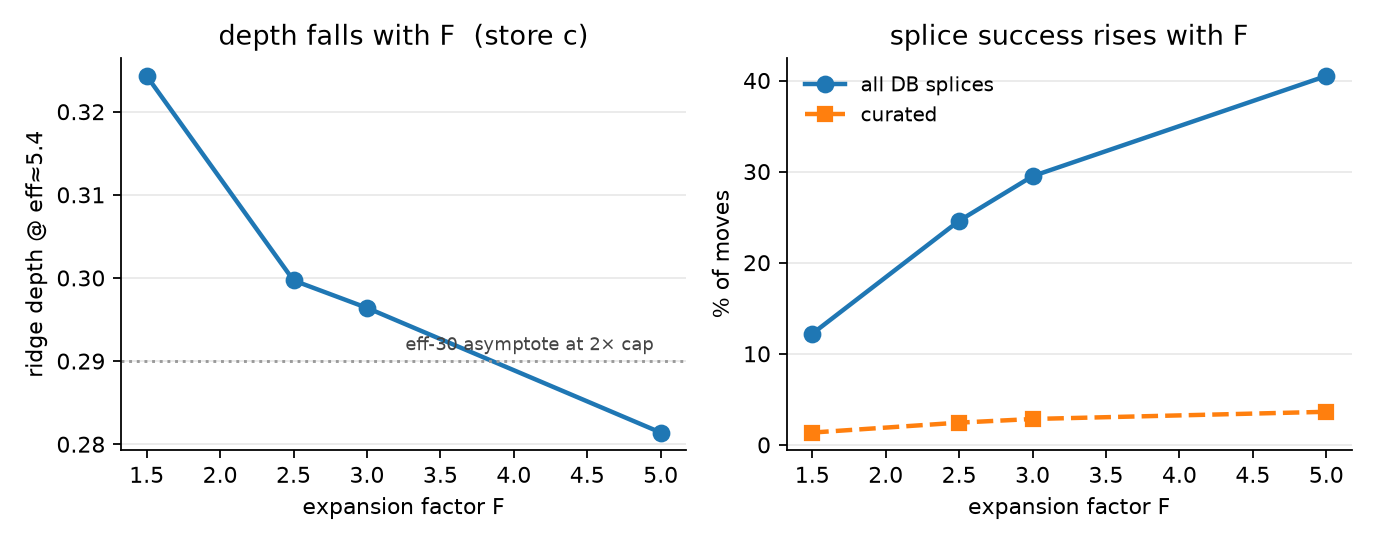
\includegraphics[width=\linewidth]{figures/factor_sweep.png}
\caption{Expansion-factor sweep on store (c): depth falls and splice
success rises monotonically with $F$.}
\end{figure}
\item \textbf{Long holds to eff 30} ($2\times$ cap, 41.9M moves/arm): (c)
and (b$'$) identical at every point ($0.314\to0.290$ vs $0.315\to0.292$),
decelerating to an asymptote ${\approx}0.290$; splice traffic decays
$23\%\to10\%$ of moves while curated's \emph{share} grows all run (b$'$:
$30\%\to49\%$ of DB splices---self-seeding, later shown causally).
\begin{figure}[H]
\centering
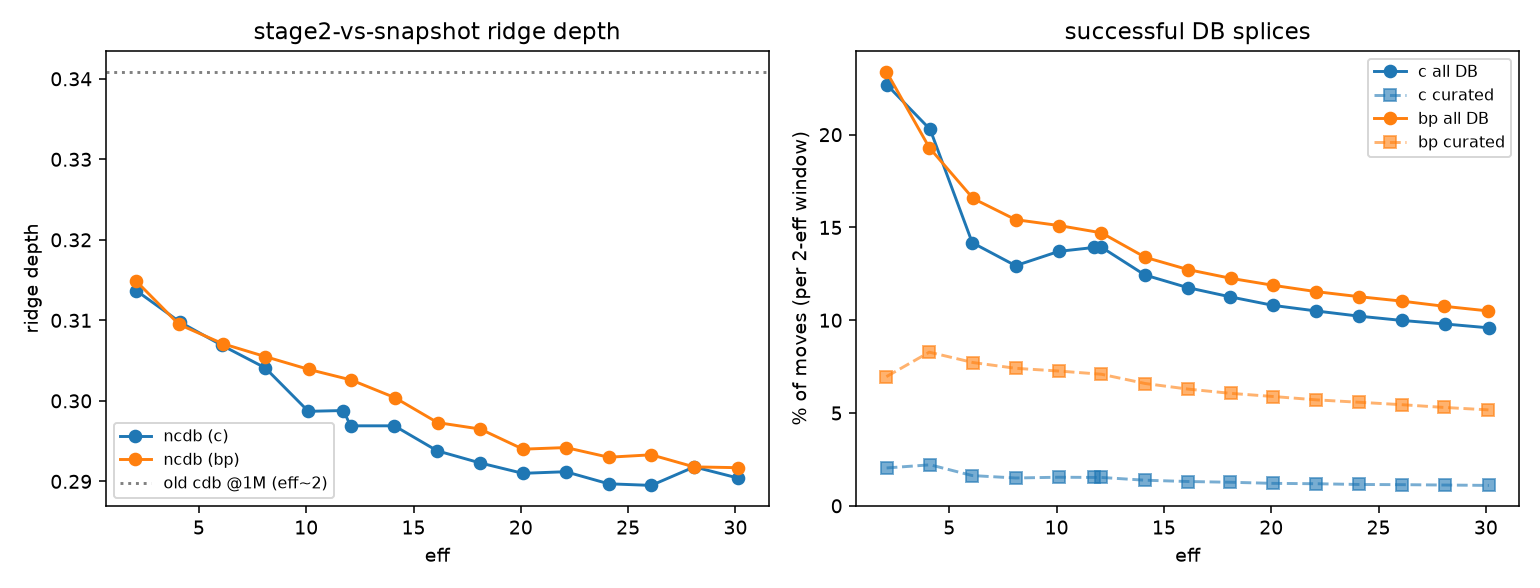
\includegraphics[width=\linewidth]{figures/long30_curves.png}
\caption{Long holds at the $2\times$ cap: ridge depth (left) and DB-splice
fraction (right) vs.\ eff for (c) and (b$'$) --- the stores never separate;
depth asymptotes near $0.290$.}
\end{figure}
\item \textbf{Ablation (peer runs, random material).} Removing the cdb
entirely---or forcing every MIX splice through it at matched splice
budget---leaves ridge depth unchanged ($\max\Delta=0.0035<$ seed spread).
\emph{Affine-ridge depth is pure dilution and is not the axis on which any
curated store differentiates}; the follow-on erasability work ties the floor
to the input's hull-erasability instead. The cdb's value therefore rests on
what these experiments did measure: correctness of served material,
certified equal-length traffic for TDP vocabulary, bounded per-key cost,
and ${\sim}50\times$ throughput.
\end{itemize}

\section{Why (c) and (b$'$)}

\begin{itemize}
\item \textbf{(a) is strictly dominated by (c).} Every (a)-pair is in (c)
with the identical per-pair guarantee; (c) additionally serves junky
keys---the common case in a mixed circuit, and the population the old store
punished with self-hits.
\item \textbf{(b) is dominated by (b$'$).} Its extra 131M pairs are
precisely friends whose small windows compress by 1--2 gates---visibly
cancellable junk (entire cohorts, e.g.\ the single-gate pool's 7-gate
friends, exist only through that hazard); no measured benefit offsets it.
\item \textbf{(c) vs (b$'$) isolates the one real dial.} Shared key policy
and small-window hygiene; they differ only in the graded leeway on spread
and large windows---strictest-certified vs maximal-certified-clean, 3.3M vs
63.1M pairs, $1\times$ vs ${\sim}5\times$ curated traffic. The interpolating
variants (v1, v2, c1) were built and measured and separate from neither
pole: storage without information.
\item \textbf{Empirically interchangeable, operationally distinct.} On
every security metric tried they tie (and the ablation result says the
ridge cannot prefer either), so the choice is structural: \textbf{(c)} for
the purest guarantee at minimal size; \textbf{(b$'$)} when curated-move
volume matters (TDP digestion, self-seeding studies, COMP-side traffic).
Both frozen stores are validated, filtered, and selectable per run via
\code{FROZEN\_CURATED\_DIR}.
\end{itemize}

\section{Artifacts}

Stores under \code{frozen\_db/}: pools \code{curated\_pools\_v3\_20260929};
composites \code{tf\_v3\_\{a,c,b,bp,v1,v2,c1\}\_*}; frozen
\code{frozen\_tf\_\{c,bp,v1,v2,c1\}\_*} with filters. Tools (working tree,
uncommitted): \code{from-frozen-identities-v3-pools}, \code{pool\_census},
\code{true\_friend\_probe} (probe + 7-mode builder + layered oracle), the
runtime circuit-key switch with tests, and the run scripts under
\code{runs/ncdb\_ab\_20261001/}. Open items: the \code{--tdp} preset stomps
\code{--no-curated*} (flag-pair workaround); store uploads to object storage
pending; the identity-function pool ($\delta=0$) stays excluded by policy.

\end{document}
